\cotefile{12}
\scanpage{137}
\[
R^{\deleted{\unsure{*}}\unsure{*|n|\bullet}}(if)_* \Leftarrow R^p i_*(R^q f_*(\mathbb Q_\ell))
\]
\diagram{\begin{tikzcd}[ampersand replacement=\&,execute at end picture={
\draw (-.42,1.05)--(3.86,1.05)--(3.92,.21)--(-.43,.29);
\draw (0,1.32)--(.04,.29);
\draw (.02,.65)--(3.85,.65);
\node[left] at (-.22,1.07) {$2$};
\node[below right] at (3.76,.21) {$N$};
\fill (1.37,1.05) circle (1.5pt);
\foreach \x in {1.36,1.52,1.60,1.96,2.29,2.59}{\fill (\x,.65) circle (1.6pt);}
\fill (2.60,.24) circle (1.7pt);
\draw[->,thick] (1.40,1.03)--(1.91,.74);
\draw[->,thick] (2.04,.57)--(2.57,.31);
}]\phantom{.}\end{tikzcd}}
avec $E^{pq}_2=0$ si $q\notin[0,2]$

\unsure{D'ailleurs|D'ailleur} $\unsure{\mathbb R|R|\mathbf R}^0 f_*(\mathbb Q_\ell)$ est essentiellement $\mathbb Q_\ell$ (au moins si $f$ à fibres connexes, auquel cas on se ramène facilement), donc les \deleted{$R^p i_*$ sont} $E^{p0}_2$ sont $(d-1)$-admissibles par \deleted{l'hyp.} ce qu'on a déjà \unsure{prouvé|vu}.

\deleted{Donc} D'autre part $R^2 f_*(\mathbb Q_\ell)\simeq\mathbb Q_\ell(-1)$, et
\[
 E^{p2}_2\simeq R^p i_*(R^2 f_*(\mathbb Q_\ell))\simeq
 \deleted{\unsure{E^{p2}_2}\ \unsure{R^p i_*}}\inserted{\mathbb Q_\ell(-1)}\otimes E^{p0}_2
\]
est donc également $(d-1)$ admissible, à fortiori \deleted{$\unsure{d+d'-1|d+d'-0}$}\inserted{$(d+d'-1)$-}admissible\inserted{ i.e. $d$-admissible}. \deleted{Pour} On en conclut, utilisant lemme 2\inserted{ et la constructibilité des $E^{pq}_2$}, que $E^{p1}_2$ \deleted{\unsure{$=$}} est une extension de \deleted{\unsure{deux}}\inserted{trois} faisceaux, les extrêmes deux \deleted{\unsure{$(d+d'-1)$-admis}} $d$-admissibles, et le médian étant $E^{p1}_3=\ldots=E^{p1}_\infty$. Il suffit donc de prouver que $E^{p1}_\infty$ est $d$-admissible, ou encore que $R^{\unsure{n|p1|p+1}}(if)_*(\mathbb Q_\ell)$ l'est, ou encore que $R^n(gf)_*(\unsure{X'|\chi'|X''})$ l'est, ce qui par Leray et lemme 3 nous ramène au cas des $R^{\unsure{-|n|\cdot}}j_*(\mathbb Q_\ell)$, qu'on sait traiter\ldots
% archive sheet number: 136
\scanpage{139}
\figure{\makebox[\linewidth][r]{
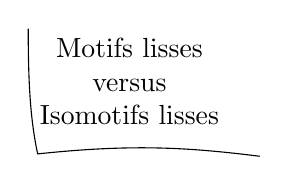
\begin{tikzpicture}
\node[align=center,anchor=north west,inner sep=4pt] at (0,0)
  {Motifs lisses\\versus\\Isomotifs lisses};
\draw (0,-.02).. controls (0,-.64) and (.02,-1.15) ..(.12,-1.61).. controls (1.35,-1.48) and (2.05,-1.53) ..(2.94,-1.64);
\end{tikzpicture}
}}
% archive sheet number: 138
\scanpage{140}
$S$ schéma normal intègre, pt générique $\eta$, $k(\eta)=K$.

\uline{Isomotif} ($\frac12$ simple) \uline{lisse} sur $S$ : = isomotif semi-simple \inserted{$M$} sur $S$, tel que pour tout $\ell\in\mathbb P$, $\ell\ne\mathrm{car}\,K$, $T_\ell(M)$ soit non ramifié rel. à $S_\ell=S[1/\ell]$

Conjecturalement, il suffit que ce soit vrai pour \uline{un} $\ell$ premier à toutes les car. résiduelles ($\Rightarrow$ il suffit que ce soit vrai pour \uline{deux} $\ell\ne\ell'$).

Motif (\unsure{isosemisimple|iso semisimple}) lisse sur $S$ (si $\mathrm{car}\,K=0$) :
\[
 =\{M,\{\mathbf{E}_\ell\},\{\alpha_\ell\}\}
\]
où

a) $M$ un isomotif lisse sur $S$

b) $\forall\,\ell$, $E_\ell$ un faisceau $\ell$-adique et tordu sur $S_\ell=S[1/\ell]$ (ou encore sur $K$, mais non ramifié rel à $S[1/\ell]$)

c) $\forall\,\ell$, $\alpha_\ell:E_\ell\deleted{\otimes_{\mathbb Z_\ell}\mathbb Q_\ell}\xrightarrow{\sim}T_\ell(M)$

avec un axiome : ``pour presque tout $\ell$, $u_\ell$ provient d'un isomorphisme sur $\mathbb Z_\ell$ -- pas seulement à torsion près''.

Ceci implique que pour \unsure{presque|\deleted{presque}} tout $\ell$, $E_\ell$ est sans torsion.

Homomorphismes de motifs lisses sur $S$
\[
 (M,\{E_\ell\}\deleted{\unsure{u\to M}},\{\alpha_\ell\})\ \unsure{\mathord{-}|\longrightarrow}\ (M',\{E'_\ell\},\{\alpha'_\ell\})
\]
donné par $(u,\{u_\ell\})$, avec $u:M-M'$ un hom de isomotifs\deleted{\unsure{de}}, et $u_\ell:E_\ell-E'_\ell$ un hom de faisceaux $\ell$-adiques tels que pour tt $\ell$, on ait commutativité de
\diagram{\begin{tikzcd}[ampersand replacement=\&]
 E_\ell\otimes_{\mathbb Z_\ell}\mathbb Q_\ell \arrow[r,dash,"\alpha_\ell"] \arrow[d,dash,"u_\ell\otimes_{\mathbb Z_\ell}\mathbb Q_\ell"] \& T_\ell(M)\arrow[d,"T_\ell(u)"]\\
 E'_\ell\otimes_{\mathbb Z_\ell}\mathbb Q_\ell \arrow[r,dash,"\alpha'_\ell"'] \& T_\ell(M')\text{ .}
\end{tikzcd}}

\uline{N.B.} Le foncteur \deleted{\unsure{Hom}} \inserted{Motifs} sur $K$ $\longleftarrow$ Motifs lisses sur $S$ est pleinement fidèle. Les Hom sont des modules de type fini sur $\mathbb Z$. La catégorie des motifs lisses sur $S$ est abélienne (on prend \uline{noyaux}, conoyaux séparément pour les composantes $M$, $E_\ell$). L\deleted{e foncteur}\inserted{'image des} \deleted{Mot} (Motifs lisses sur $S$) \unsure{en|dans|$\to$} (Motifs sur $K$) est une ss-catégorie abélienne \uline{épaisse}.

Le foncteur $(\text{Motifs}\inserted{\text{ lisses}})\to(\text{Isomotifs}\inserted{\text{ lisses}})$ est exact ess\textsuperscript{t} surjectif
% archive sheet number: 139
\scanpage{141}
La catégorie des groupes finis \inserted{comm. $G$} sur $K$ tel que pour tt $\ell$, $G(\ell)$ soit non ramifié rel. à $S[1/\ell]$, est une sous catégorie épaisse de celle des motifs sur $S$, la catégorie quotient est équivalente à celle des isomotifs lisses sur $S$.

La catégorie des motifs est une $\otimes$-catégorie avec \uline{Hom}. Les foncteurs motifs $\longrightarrow$ isomotifs, motifs $\to$ faisceaux $\ell$-adiques, sont des $\otimes$-foncteurs, compatibles aux \uline{Hom}.

Un \deleted{définit} hom de motifs est une isogénie s'il induit un isom sur les isomotifs sousjacents. On définit la dimension (ou le poids), le niveau etc en termes des isomotifs.

Tout schéma propre et lisse $X$ sur $S$ définit des motifs\inserted{ sur $S$}, notés $R^i f_*(\mathbb Z_X)$ s'il n'y a pas de confusion à craindre. de $=$ pour des \unsure{sites} étales relatifs lisses et propres.

\uline{Relations avec les schémas en groupes commutatifs propres et lisses}.

On définit un foncteur \uline{contravariant} de la catégorie de ces objets, soit $A$, dans la catégorie des motifs sur $S$, en posant
\[
\begin{aligned}
&\deleted{\unsure{\Phi|\varphi|\mathfrak P}(A)=R^1 f_*(\mathbb Z_A)=\bigl(\ R^1 f_*(\bigr.}\\
&\Phi(A)=(M,E_\ell,u)
\end{aligned}
\]
où
\[
\left\{\begin{aligned}
 M&=R^1(f_{A^0})_*(\mathbb Q_{A^0})\\
 E_\ell&=\underline{\operatorname{Hom}}({}_{\ell^\infty}A,\mathbb Q_\ell/\mathbb Z_\ell)\\
 &u_\ell\ \text{provenant de l'hom évident}\\
 &\hspace{4em}E_\ell\longrightarrow R^1 f_{A^0*}(\mathbb Z_{\ell A^0})
\end{aligned}\right.
\]
\margin{extension de $\underline{\operatorname{Hom}}(A/A^0,\mathbb Q_\ell/\mathbb Z_\ell\unsure{)}$ par $R^1 f_{A^0*}(\mathbb Z_{\ell A^0})$}

\uline{NB} Il suffirait que $A$ \deleted{\unsure{soit|soit un} \unsure{à supp.|extension}} \inserted{soit extension d'un schéma} en gr fini $A/A^0$ par un schéma abélien $A^0$, avec $A/A^0(\ell)$ extension par $0$ d'un groupe fini étale sur $S_\ell\deleted{\unsure{0}}$.
% archive sheet number: 140
\scanpage{142}
\uline{Le foncteur} $\Phi$ \uline{est pleinement fidèle} (On est ramené au cas de la base $\eta=\operatorname{Spec}K$).

L'image essentielle est \deleted{\uline{\unsure{contenue}} dans} formée des motifs $(M,\{E_\ell\},\{u_\ell\})$ tels que \deleted{les $E_\ell$} leur quotient modulo torsion soit associé à un \uline{schéma} \uline{abélien} sur $S$.

Il \uline{faut} \uline{\unsure{pour|voir}} cela que $M$ soit effectif de poids $1$, i.e. soit défini par un schéma abélien \inserted{$A_K$} sur $K$. \deleted{\unsure{Il} \unsure{Mais}}

La question si cette \unsure{question|condition} est suffisante revient à celle-ci : Soit $A$ un schéma abélien sur $K$, \deleted{de} tel que $\forall\,\ell$, \deleted{les} $T_\ell(A)$ soit non ramifié sur $S_\ell$, alors $A$ a bonne réduction sur $S$. Cela marche si $S$ est de dim $1$\inserted{ (critère de \inserted{\unsure{Néron}-}Ogg-\unsure{Chafarevitch|Chafarévitch|Chafarevich})}, \uline{ou} si $S$ de car. nulle (critère de \unsure{mézigues}), mais peut-être pas en général (p.ex. anneau local régulier de dim $2$ d'inégales caractéristiques). Pour faire un contre-exemple, il suffirait d'avoir un exemple d'un schéma abélien $A$ sur $S$, et d'un ss-groupe fini de $A_K$ qui ne se prolonge pas en un ss-groupe \uline{fini} et \uline{plat} de $A$. S'il y avait un tel exemple, il y en aurait aussi avec un ordre premier.....

\margin{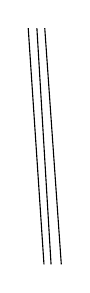
\begin{tikzpicture}[x=1mm,y=1mm]\draw (0,30)--(2,0) (1.1,30)--(2.9,0) (2.1,30)--(4.2,0);\end{tikzpicture}}
\uline{Pb} Avec la définition adoptée de motif lisse (en termes de celle de isomotif lisse, comme un isomotif \uline{sur} $K$ avec simplement une propriété \inserted{``galoisienne''} de non ramification pour les $T_\ell$) il n'est pas du tout \unsure{claire|clair} comment définir l'image inverse d'un motif (resp. d'un isomotif) par $S'\unsure{\mathord{-}|\to}S$, p.ex. des fibres en les $s\in S$. Cette difficulté \deleted{\unsure{se pose}}\inserted{concerne} en fait les isomotifs, et vaut déjà pour ceux qui sont effectifs de poids $1$.
% archive sheet number: 141
\scanpage{143}
\begin{flushright}\begin{minipage}{0.46\linewidth}\raggedright
Enveloppes pseudo-abéliennes\unsure{.}\\
de catégories multiplicatives\\
(\unsure{Constructions|Construction} abstraites de\\
Catégories de motifs).
\end{minipage}\end{flushright}
% archive sheet number: 142
\scanpage{144}
\uline{Construction abstraite d'une théorie de motifs semi-simples.}

On part d'une catégorie $\mathscr V$ \deleted{\unsure{pré}}``additive'', \deleted{\unsure{i.e. où}}\inserted{en particulier} les \deleted{Hom}\inserted{Fl}$(X,Y)$ \deleted{sont} munis d'une structure de groupe abélien, les accouplements de composition étant bilinéaires. \deleted{[On ne suppose pas qu'il existe un objet nul, ni des sommes \unsure{ou} produits de deux objets .....]} On s'intéresse, pour toute catégorie \uline{abélienne} $\mathcal C$, aux foncteurs \deleted{contravariants} ``additifs'' (i.e. commutant aux sommes finies, \unsure{ou ce qui revient au|ou encore} $=$, aux produits finis)
\[
 H\deleted{\unsure{F}}:\mathscr V^{\deleted{\unsure{\circ|*}}}\longrightarrow\mathcal C
\]
et on cherche un foncteur universel de cette nature
\[
 \underline{h}:\mathscr V^{\deleted{\circ}}\longrightarrow\mathcal M(\mathscr V)=\mathcal M
\]
foncteur additif dans catégorie abélienne $\mathcal M$) tel que pour toute catégorie abélienne $\mathcal C$, l'application
\[
\begin{aligned}
 T&\mapsto T\circ\underline h\\
 \operatorname{Fonc\,exacts}(\mathcal M,\mathcal C)&\longrightarrow\operatorname{Fonc\,add}(\mathscr V^{\deleted{\circ}},\mathcal C)
\end{aligned}
\]
soit bijective (ce qui caractériserait $\mathcal M$ à \deleted{\unsure{équivalence}} isom près), ou le cas échéant, que
\[
 \underline{\operatorname{Fonc\,exacts}}(\mathcal M,\mathcal C)\ \unsure{\mathord{-}|\longrightarrow}\ \underline{\operatorname{Fonc\,add}}(\mathscr V^{\deleted{\circ}},\mathcal C)
\]
soit une équivalence de catégories (ce qui
% archive sheet number: 143
\scanpage{145}
caractérisera $\mathcal M$ à équivalence près). De plus, on aime donner des conditions moyennant lesquelles le foncteur $\underline h$ est \uline{pleinement fidèle}.

On va supposer que la structure \deleted{\unsure{pré}}additive sur $\mathscr V$ peut s'enrichir en une structure $k$-linéaire, où $\deleted{\unsure{k}}Q$ est un \uline{corps} commutatif,
% slanted
\margin{i.e. on a un hom d'anneaux $Q\to\operatorname{End}\,\mathrm{id}_{\mathscr V}$}
[NB. si $Q=\mathbb Q$, cet enrichissement est déterminé de façon unique]. On suppose que \deleted{les \unsure{Hom} $\operatorname{Fl}(X,Y)$ sont des \unsure{esp vectoriels|espaces vectoriels} de dim finie sur $k$, et} que pour tt $X$, $\operatorname{Fl}(X,X)$ est une \uline{algèbre} \inserted{\uline{de degré fini}} \uline{semi-simple} sur $\deleted{\unsure{k}}Q$. Nous allons alors \deleted{\unsure{de|en}} construire une catégorie $\mathcal M^{\deleted{\unsure{\circ|0|\#}}}$ de la façon suivante. Un objet de $\mathcal M^{\deleted{\circ}}$ est un couple $(X,\pi)$, où $X\in\operatorname{Ob}\mathscr V$, $\pi\in\operatorname{Fl}(X,X)$, $\pi^2=\pi$ ($\pi$ est un \uline{projecteur} de $X$). Un homomorphisme $(X,\pi)\to(X',\pi')$ est un hom $f:X\to X'$ tel que $\pi'f=f\pi$, \uline{modulo} les $f$ tels que $f\pi=\pi'f=0$.
\diagram{\begin{tikzcd}[ampersand replacement=\&,row sep=small,column sep=small]
X\arrow[r,dash,"\pi"]\arrow[d,"f"'] \& X\arrow[d,"f"]\\
X'\arrow[r,dash,"\pi'"]\arrow[d,"g"'] \& X'\arrow[d,"g"]\\
X''\arrow[r,dash,"\pi''"] \& X''
\end{tikzcd}}
On compose de façon évidente. D'où une catégorie\inserted{ $\mathcal M^{\deleted{\circ}}$}, manifestement additive, et un foncteur additif
% archive sheet number: 144
\scanpage{146}
évident, d'ailleurs pleinement fidèle
\[
 \underline h^{\deleted{\unsure{\circ|0|\#}}}:\mathscr V\longrightarrow\mathcal M^{\deleted{\circ}}
\]
en posant $\underline h^{\deleted{\circ}}(X)=(X,\mathrm{id}_X)$. Pour toute catégorie abélienne\inserted{ $\mathcal C$},
% slanted
\margin{il suffit que $\mathcal C$ soit une catégorie additive où les projecteurs sont réalisables}
le foncteur $\varphi:T\mapsto T\circ h$
\[
 \underline{\operatorname{Fonc\,add}}(\mathcal M,\mathcal C)\xrightarrow{\varphi}\underline{\operatorname{Fonc\,add}}(\mathscr V,\mathcal C)
\]
est une \deleted{isomorphisme} équivalence. Pour le voir, on va construire un foncteur quasi-inverse \deleted{1°) pleinement fidèle. Un}
\[
 \psi:\underline{\operatorname{Fonc\,add}}(\mathscr V,\mathcal C)\longrightarrow\underline{\operatorname{Fonc\,add}}(\mathcal M,\mathcal C)
\]
en associant à \unsure{tout|tt} foncteur\inserted{ additif} $H:\mathscr V\unsure{\mathord{-}|\to}\mathcal C$ son extension canonique
\[
 \psi(H)(X,\pi)=\operatorname{Im}H(\pi)
\]
avec la loi fonctorielle évidente. On voit aussitôt que l'on a des isom can
\[
\begin{aligned}
 \varphi\deleted{\unsure{(}}\psi\deleted{\unsure{)}}(H)&\simeq H\\
 \psi\varphi(T)&\simeq T
\end{aligned}
\]

Pour l'instant, cette construction et propriété universelle de $\mathcal M$ n'utilise pas les hyp particulières faites sur $\mathscr V$ ; elle répond au Pb universel de rendre \uline{tous les projecteurs réalisables}.\inserted{ (ds catégorie additive donnée)} Mais les hypothèses faites sur $\mathscr V$ vont impliquer que $\mathcal M$ est en fait une catégorie \inserted{\uline{abélienne}} \uline{semi-simple} (i.e. tout objet de
% archive sheet number: 145
\scanpage{147}
permet de \unsure{nous|les|se} ramener à un objet $P$ de la forme $\underline h(X)$, \deleted{\unsure{donc|dans} $u$ de la forme $\underline h(\alpha)$, où $\alpha\in\operatorname{Fl}(X,X)$. Or comme} \inserted{$\operatorname{Fl}(P,P)\simeq\operatorname{Fl}(X,X)$, donc} $\operatorname{Fl}(\deleted{\unsure{X}}P,\deleted{\unsure{X}}P)$ est un \uline{anneau semi-simple} $U$, \deleted{Or}

\deleted{Pour un tel anneau, \unsure{dont} il est \unsure{opérant} sur un objet d'une catégorie} \deleted{Alors $P$ et $u$ se décomposent suivant les composantes simples de $U=\operatorname{Fl}(P,P)$ (i.e. de son centre) et \unsure{on est ramené au cas où les}}

Or lorsque un anneau de ce type opère sur un objet d'une catégorie abélienne, alors pour tout $u\in U$, on peut trouver \deleted{deux couples d'\unsure{idempotents} orthogonaux complémentaires $\pi,\pi'$ de $U$, \unsure{tels que} $(\pi\pi'=\pi'\pi=0,\ \pi+\pi'=1,\ \pi^2=\pi,\ \pi'^2=\pi')$ tels que et $\varpi,\varpi'$ tels que $u\pi'=0,\varpi'u=0$,} $v\in U$ tel que
\[
\begin{aligned}
 vu&\ \text{soit un }\deleted{\text{projecteur}}\inserted{\text{\unsure{idem.pot|idempot|idempotent}}}\ \pi\\
 uv&\ \text{soit}\ \rule{2.5cm}{0.35pt}\ \varpi
\end{aligned}
\]
\begin{tikzpicture}[baseline=(phrase.base)]
\node[anchor=west,inner sep=0pt] (phrase) at (0,0) {et on ait les relations};
\node[draw,ellipse,inner sep=2pt] (relations) at (-0.3,-1.1) {\inserted{$\begin{aligned}\pi v&=v,\ u\pi=u\\\varpi u&=u,\ v\varpi=v\end{aligned}$}};
\draw[->] (relations.north east) .. controls +(0.5,0.5) and +(0.1,-0.7) .. (phrase.east);
\end{tikzpicture}

\diagram{\begin{tikzcd}[ampersand replacement=\&,row sep=small]
 P\simeq\pi P\unsure{+|\oplus}\pi'P \arrow[dr] \&\\
 \& \pi P\arrow[d,"\sim"]\\
 Q\simeq\varpi Q+\varpi'Q \& \varpi Q\arrow[l]
\end{tikzcd}}

\diagram{\begin{tikzcd}[ampersand replacement=\&,column sep=small,row sep=small]
P\arrow[r,"u",very thick]\arrow[d] \& \deleted{\unsure{P}}Q\arrow[l,bend right=38,"v"']\\
P'\arrow[r,"\sim"] \& Q'\arrow[u]
\end{tikzcd}}
\[
\left\{\begin{aligned}
 vu&=\text{projecteur }\pi,\\
 uv&=\text{projecteur }\varpi,\\
 &\deleted{\unsure{\varpi u}}
\end{aligned}\right.
\]
de cette façon, on gagne donc.

\diagram{\begin{tikzcd}[ampersand replacement=\&,column sep=small,row sep=small]
 P'+P''\arrow[dr] \& \& \& Q'+Q''\arrow[dl]\\
 \& P'\arrow[ul,shift right=1.6pt]\arrow[ul,shift left=4pt]\arrow[r,shift right=2pt,very thick] \& Q'\arrow[l,shift right=2pt]\arrow[ur,shift right=2pt] \&
\end{tikzcd}}
Pour les conditions de chaînes, on utilise le fait que les $\operatorname{Fl}(X,X)$ sont de \deleted{degré} dim finie sur $k$. ....
% archive sheet number: 146
\scanpage{148}
cette catégorie est semi-simple). Si alors $\mathcal C$ est une catégorie abélienne, les foncteurs additifs de $\mathcal M$ dans $\mathcal C$ sont autom. exacts. Cela prouve que le ``Pb universel''\inserted{ (avec grain de sel)} en termes de catégories abéliennes (Variante $2$) est résolu par $\mathcal M$.

Prouvons donc que $\mathcal M$ est une catégorie \uline{abélienne semi-simple}. Cela équivaut à ceci :

\deleted{tout morphisme est \unsure{sa}}

(i) Tout objet\deleted{\unsure{X}} satisfait condition des chaînes ascend\textsuperscript{tes}, et descendantes pour les sous-objets facteurs directs,

\deleted{i.e. l'ens des \unsure{fa}}

(ii) Tout morphisme $u:P\longrightarrow Q$ est ``direct'', i.e. isom à un morphisme
\[
 A\times B\xrightarrow[\operatorname{inj}_1\circ\operatorname{pr}_2]{}B\times C
\]

Pour vérifier (ii), \deleted{\unsure{supposons}} considérons $R=P\times Q$, et l'endomorphisme \deleted{$\unsure{\operatorname{pr}_2|\operatorname{pr}_1}$} $v=\operatorname{inj}_2\,u\operatorname{pr}_2$ de $R$. On voit aisément que pour \deleted{\unsure{que}} (ii)\inserted{ soit vrai} pour $u$, il\inserted{ \unsure{f.|faut} et} suffit \deleted{\unsure{de}} qu'il le soit pour $v$, donc on est ramené au cas où $P=Q$.
% slanted
\margin{donner lemme \unsure{commun|connexe} : il est innocent de modifier $P\to Q$ par
\diagram{\begin{tikzcd}[ampersand replacement=\&,column sep=small,row sep=small]
 P+P'\arrow[d] \& Q+Q'\arrow[dl,bend left=20]\\
 P\arrow[r] \& Q\arrow[u]
\end{tikzcd}}}
D'autre part, soit \deleted{\unsure{R}} $S$ un autre objet, et \unsure{sur|soit} $R=P+S$, $v=u\oplus\deleted{\unsure{1|\mathrm{id}}}0_S$, alors on constate que la propriété est vraie pour $u$ ssi elle l'est pour $v$. Cela nous
% archive sheet number: 147
\scanpage{149}
On suppose donné trois catégories \inserted{additives} $\mathscr V,\mathscr V',\mathscr V''$, d'où $\mathcal M,\mathcal M',\mathcal M''$, on suppose donné un foncteur biadditif $\mathscr V\times\mathscr V'\unsure{\mathord{-}|\longrightarrow}\mathscr V''$. Alors il se prolonge de façon ess\textsuperscript{t} unique en un foncteur bi-additif $\mathcal M\times\mathcal M'-\mathcal M''$. En fait, \unsure{on|ce} voit que la propriété \inserted{pseudo-}universelle qui définit $\mathcal M$ en terme de $\mathscr V$, s'étend aux bifoncteurs, ......

On \deleted{\unsure{y}} utilisera cette construction surtout pour un bifoncteur $\mathscr V\times\mathscr V-\mathscr V$ ``\uline{symétrique}'', et ``\uline{associatif}''\inserted{ et ``unitaire''}, noté $\deleted{\otimes}\boxtimes$. Alors on trouve un bifoncteur de $=$ nature dans $\mathcal M$, noté $\otimes$. Si $k$ est \uline{de car. $0$}\inserted{ (p.ex. $\mathbb Q$)}, on peut construire alors toutes les opérations tensorielles\inserted{ covariantes} dans $\mathcal M$ [en plusieurs arguments], par exemple on pourra définir les
\[
 \overset{\unsure{n|-}}{\bigotimes} M,\quad \overset{n}{\bigwedge}M,\quad\deleted{\text{etc}}\ S^n(M)\quad\text{etc ....}
\]
% archive sheet number: 148
